%%%%%%%%%%%%%%%%%%%%%%%%%%%%%%%%%%%%%%%%%
% Beamer Presentation
% LaTeX Template
% Version 1.0 (10/11/12)
%
% This template has been downloaded from:
% http://www.LaTeXTemplates.com
%
% License:
% CC BY-NC-SA 3.0 (http://creativecommons.org/licenses/by-nc-sa/3.0/)
%
%%%%%%%%%%%%%%%%%%%%%%%%%%%%%%%%%%%%%%%%%

%----------------------------------------------------------------------------------------
%	PACKAGES AND THEMES
%----------------------------------------------------------------------------------------

\documentclass[xcolor=table, envcountsect,12pt]{beamer}
\setbeamertemplate{theorems}[numbered]
\mode<presentation> {
	
	% The Beamer class comes with a number of default slide themes
	% which change the colors and layouts of slides. Below this is a list
	% of all the themes, uncomment each in turn to see what they look like.
	
	%\usetheme{default}
	%\usetheme{AnnArbor}
	%\usetheme{Antibes}
	%\usetheme{Bergen}
	%\usetheme{Berkeley} %
	%\usetheme{Berlin} %
	%\usetheme{Boadilla}
	%\usetheme{CambridgeUS} %
	%\usetheme{Copenhagen}
	%\usetheme{Darmstadt}
	%\usetheme{Dresden} %
	%\usetheme{Frankfurt}
	%\usetheme{Goettingen}
	%\usetheme{Hannover}
	\usetheme{Ilmenau} %
	%\usetheme{JuanLesPins}
	%\usetheme{Luebeck}
	%\usetheme{Madrid}
	%\usetheme{Malmoe}
	%\usetheme{Marburg}
	%\usetheme{Montpellier}
	%\usetheme{PaloAlto} %
	%\usetheme{Pittsburgh}
	%\usetheme{Rochester}
	%\usetheme{Singapore}
	%\usetheme{Szeged}
	%\usetheme{Warsaw}
	
	% As well as themes, the Beamer class has a number of color themes
	% for any slide theme. Uncomment each of these in turn to see how it
	% changes the colors of your current slide theme.
	
	%\usecolortheme{albatross}
	%\usecolortheme{beaver}
	%\usecolortheme{beetle}
	%\usecolortheme{crane}
	%\usecolortheme{dolphin}
	%\usecolortheme{dove}
	%\usecolortheme{fly}
	%\usecolortheme{lily}
	%\usecolortheme{orchid}
	%\usecolortheme{rose}
	%\usecolortheme{seagull}
	%\usecolortheme{seahorse}
	%\usecolortheme{whale}
	%\usecolortheme{wolverine}
	
	%\setbeamertemplate{footline} % To remove the footer line in all slides uncomment this line
	%\setbeamertemplate{footline}[page number] % To replace the footer line in all slides with a simple slide count uncomment this line
	\setbeamertemplate{footline}[text line]{%
  		\parbox{\linewidth}{\vspace*{-8pt}Graduate Student Seminar\hfill\insertshortauthor\hfill\insertshorttitle}}
	\setbeamertemplate{navigation symbols}{} % To remove the navigation symbols from the bottom of all slides uncomment this line
}
\usepackage{etex}

%%--
\usepackage{graphicx} % Allows including images
\usepackage{booktabs} % Allows the use of \toprule, \midrule and \bottomrule in tables
%%--
\usepackage{url}
\usepackage{soul}
\usepackage{xcolor}
\usepackage{lipsum}
\usepackage[normalem]{ulem}
\usepackage{amsmath}
\usepackage{amsthm}
\usepackage{amssymb}
\usepackage{dsfont}
\usepackage{bbm}
\usepackage{graphicx}
\usepackage{epstopdf}
\usepackage{multicol}
\usepackage{multirow}
\usepackage{color}
\usepackage{threeparttable}
\usepackage{caption}
\usepackage{subcaption}
\captionsetup{compatibility=false}
\DeclareMathOperator*{\argmax}{arg\,max}
\theoremstyle{remark}
\newtheorem*{rem}{Remark}
\theoremstyle{theorem}
\newtheorem{prop}{Proposition}
\usepackage{pdflscape}
\usepackage{afterpage}
\setcounter{MaxMatrixCols}{34}
\usepackage{dcolumn}
\usepackage{geometry}
\usepackage{tikz}
\usetikzlibrary{shapes.arrows, positioning}
%%-----------------------------------------------------------------------------------
\makeatletter
%%%%%%%%%%%%% Textclass specific LaTeX commands.
%\makeatletter
\theoremstyle{plain}
\newtheorem{lem}{Lemma}
\newtheorem{cor}{Corollary}
\newtheorem{conjecture}{Conjecture}
%%
\makeatletter
\beamer@theme@subsectionfalse
\makeatother
%
%CUSTOM COMMAND FOR BLUE URLs
\newcommand{\myul}[2][black]{\setulcolor{#1}\ul{#2}\setulcolor{black}}

% bibliography
\input{biblatex-aer}
\renewcommand{\bibfont}{\tiny}
\addbibresource{references.bib}

%
%
%-----------------------------------------------------------------------------------------
%----------------------------------------------------------------------------------------
%	TITLE PAGE INFO
%----------------------------------------------------------------------------------------
\title{Liquidity Shocks in Virtual Markets}
\author{Caleb Bray}
\date{August 24, 2026}
\vspace{.2in}

%------------------------------------------------
\begin{document}
	% title page
	\begin{frame}
		\titlepage
	\end{frame}

	
	
%--------------------------------------------------------------------------------------------------
%	INTRODUCTION
%--------------------------------------------------------------------------------------------------
\section{Introduction}

\begin{frame}[shrink=3]{Introduction}
	\begin{itemize}
		\item \footnotesize This paper serves as a case study to estimate the effects of sudden market structure changes in virtual asset markets.
		\item \footnotesize In particular, I look at the market for cosmetics (AKA ``skins'') in the video games Counter-Strike and Dota 2.
		\begin{itemize}
			\item \scriptsize The market for these items is surprisingly large: Counter-Strike hit a market capitalization of \$4.3 billion in March 2025 \autocite{bloomberg2025-03-07}.
			\item \scriptsize On 3/29/18, all Counter-Strike items were trade restricted, preventing sale \& trade within 7 days of acquisition. This restriction continues today and was not applied to Dota 2 items until May 2020.
		\end{itemize}
		\item \footnotesize I use a DID specification to identify a 4.2\% decrease in quality-adjusted prices and 34.4\% drop in trade volume after implementation of a 7-day trade ban on a subset of items listed on a virtual exchange.
		\begin{itemize}
			\item \scriptsize Overall, the treated items maintained a higher price level than the untreated items, suggesting that these items retained their amenity value but lost investment value causing a dip in quality-adjusted prices.
			\item \scriptsize This effect manifests as a downward level shift that remains significant for over a year post-treatment despite the growing number of users, and is consistent with empirical findings in the literature.
		\end{itemize}
	\end{itemize}
\end{frame}

\begin{frame}[shrink=20]{Contribution}
	\begin{itemize}
		\item \footnotesize  \textbf{Treasuries \& OTC Markets:} Trade delays and market driven declines in liquidity have meaningful effects on asset price and choice \parencites{dgp_2005}{dgp_2007}{krishna_2002}{lagos_rocheteau_2007}{amihud_et_al_2006}{geromichalos_et_al_2016}.
		\begin{itemize}
			\item \footnotesize  \textcolor{red}{\textbf{Contribution:} I study a fixed top-down implementation of an exogenous trade delay, allowing me directly observe the liquidity premium.}
		\end{itemize}
		\item \footnotesize  \textbf{Hedonic Pricing:} Unquantifiable properties intrinsic to goods (aesthetics, location, etc.) play an important role in pricing and consumer choice \parencites{lancaster_1966}{rosen_1974}{rosen1986}{sirmans_2005}.
		\begin{itemize}
			\item \footnotesize  \textcolor{red}{\textbf{Contribution:} I show this applies to virtual assets designed and governed by a singular entity. In this case, the price is largely driven by these aesthetic features.}
		\end{itemize}
		\item \footnotesize  \textbf{Alternative Digital Assets:} As assets, Counter-Strike skins experience sizable returns, with average annual returns of 40\% and low exposure to traditional financial markets. Lower financial returns on expensive skins are likely compensated by the ``emotional dividend'' of gamers \parencite{dobrynskaya_2025}.
		\begin{itemize}
			\item \footnotesize \textcolor{red}{\textbf{Contribution:} I show that the emotional dividend is large as most of the skins' value is retained. I show that market structure is incredibly relevant for the growing number of virtual exchanges (eg: P2P Crypto Exchanges).}
		\end{itemize}
	\end{itemize}
\end{frame}

%--------------------------------------------------------------------------------------------------
%	INSTITUTIONAL DETAILS
%--------------------------------------------------------------------------------------------------
\section{Institutional Details}

\begin{frame}{Skins Overview}
\begin{center}
\vspace{-4mm}
\begin{tikzpicture}[
    every node/.style={inner sep=0pt}
]
    % Top image
    \node (img1) {
        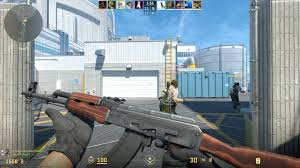
\includegraphics[scale=0.45]{default_ak.jpg}
    };
    
    % Bottom image (smaller gap)
    \node[below=2cm of img1] (img2) {
        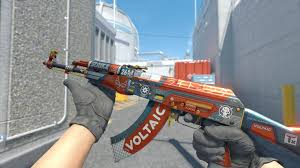
\includegraphics[scale=0.45]{bloodsport_ak.jpg}
    };
    
    % Middle point
    \path (img1.south) -- (img2.north) coordinate[midway] (middle);
    
    % Downward arrow with wider body
    \node[
        single arrow,
        draw=black,
        fill=black,
        minimum height=2cm,
        minimum width=0.3cm,
        single arrow head extend=0.1cm,
        single arrow tip angle=90,
        anchor=center,
        rotate=-90,
        inner sep=0.3cm
    ] (arrow) at ([yshift=0.15cm]middle) {};
    
    % Overlay image (shifted up 0.3cm)
    \node at (arrow.center) {
        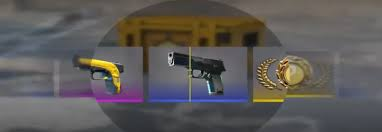
\includegraphics[scale=0.25]{case_opening.jpg}
    };
\end{tikzpicture}
\qquad
\begin{tikzpicture}[
    every node/.style={inner sep=0pt}
]
    % Top image
    \node (img1) {
        
\includegraphics[scale=0.06]{default_invoker.png}
    };
    
    % Bottom image (smaller gap)
    \node[below=2cm of img1] (img2) {
        
\includegraphics[scale=0.105]{skin_invoker.png}
    };
    
    % Middle point
    \path (img1.south) -- (img2.north) coordinate[midway] (middle);
    
    % Downward arrow with wider body
    \node[
        single arrow,
        draw=black,
        fill=black,
        minimum height=2cm,
        minimum width=0.3cm,
        single arrow head extend=0.1cm,
        single arrow tip angle=90,
        anchor=center,
        rotate=-90,
        inner sep=0.3cm
    ] (arrow) at ([yshift=0.15cm]middle) {};
    
    % Overlay image (shifted up 0.3cm)
    \node at (arrow.center) {
        
\includegraphics[scale=0.22]{dota2_treasure.jpg}
    };
\end{tikzpicture}
\end{center}
\end{frame}

\begin{frame}{The Marketplaces}
    \begin{figure}[ht]
        \begin{minipage}[b]{0.45\linewidth}
            \centering
            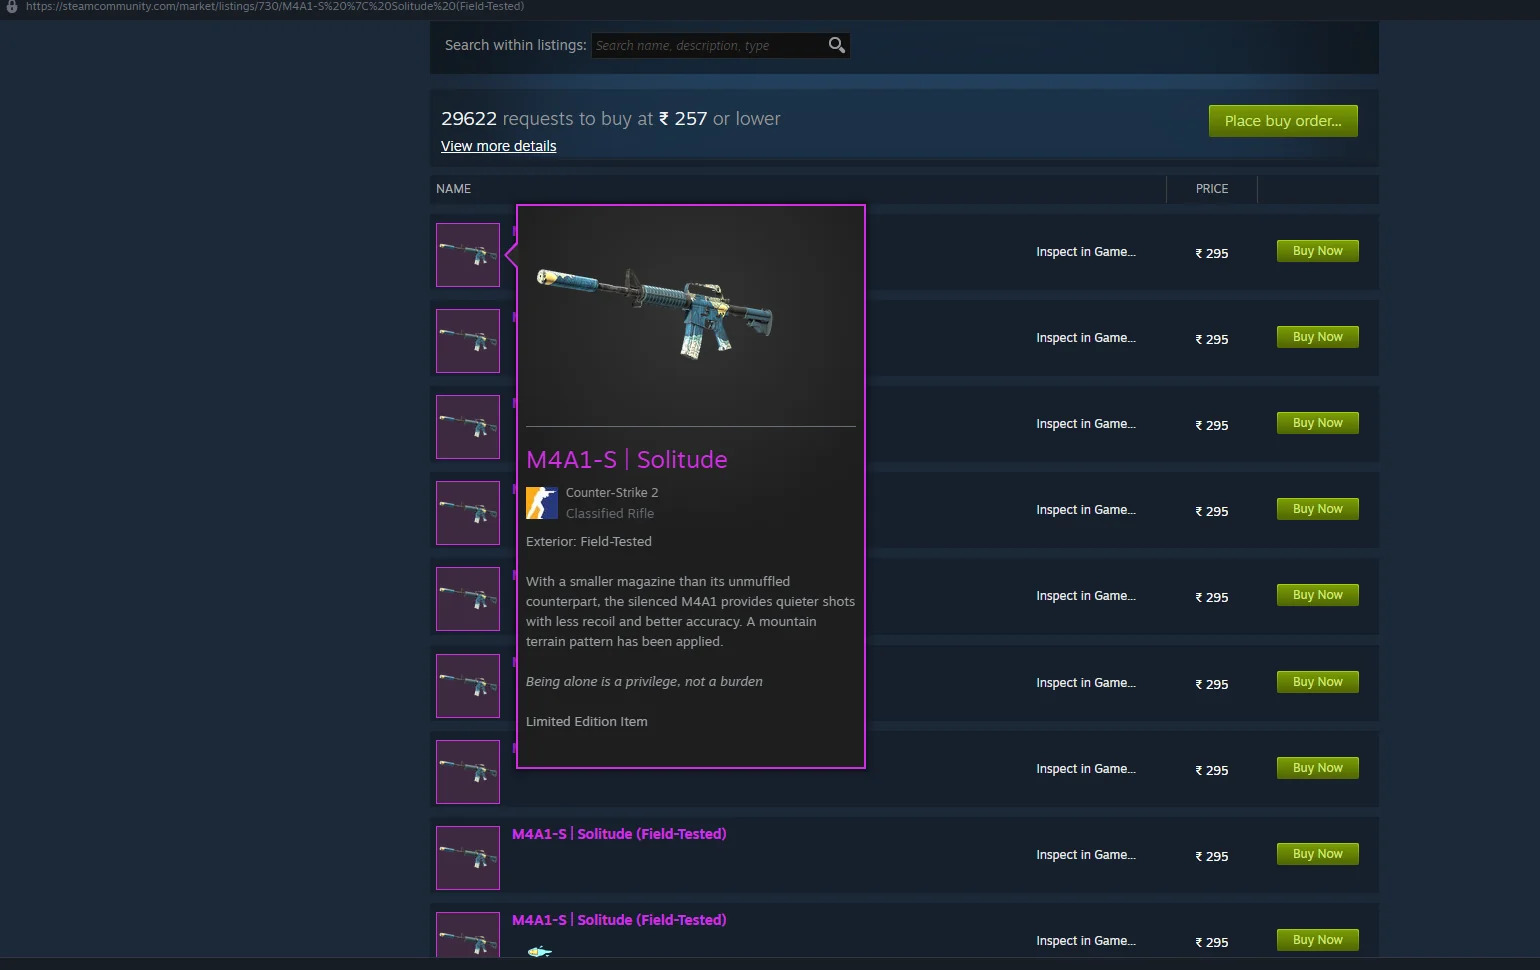
\includegraphics[width=5.1cm,height=3.7cm]{market_listing.jpg}
            \footnotesize Steam Community Market Listings
        \end{minipage}
        \hspace{0.5cm}
        \begin{minipage}[b]{0.45\linewidth}
            \centering
            
\includegraphics[width=5.1cm,height=3.7cm]{skinport.jpg}
            \footnotesize Trade with a Third-Party Bot Account
        \end{minipage}
    \end{figure}
\end{frame}

\begin{frame}{The 3/29/18 Trade Ban}
	\begin{figure}
		\centering
		\makebox[0pt]{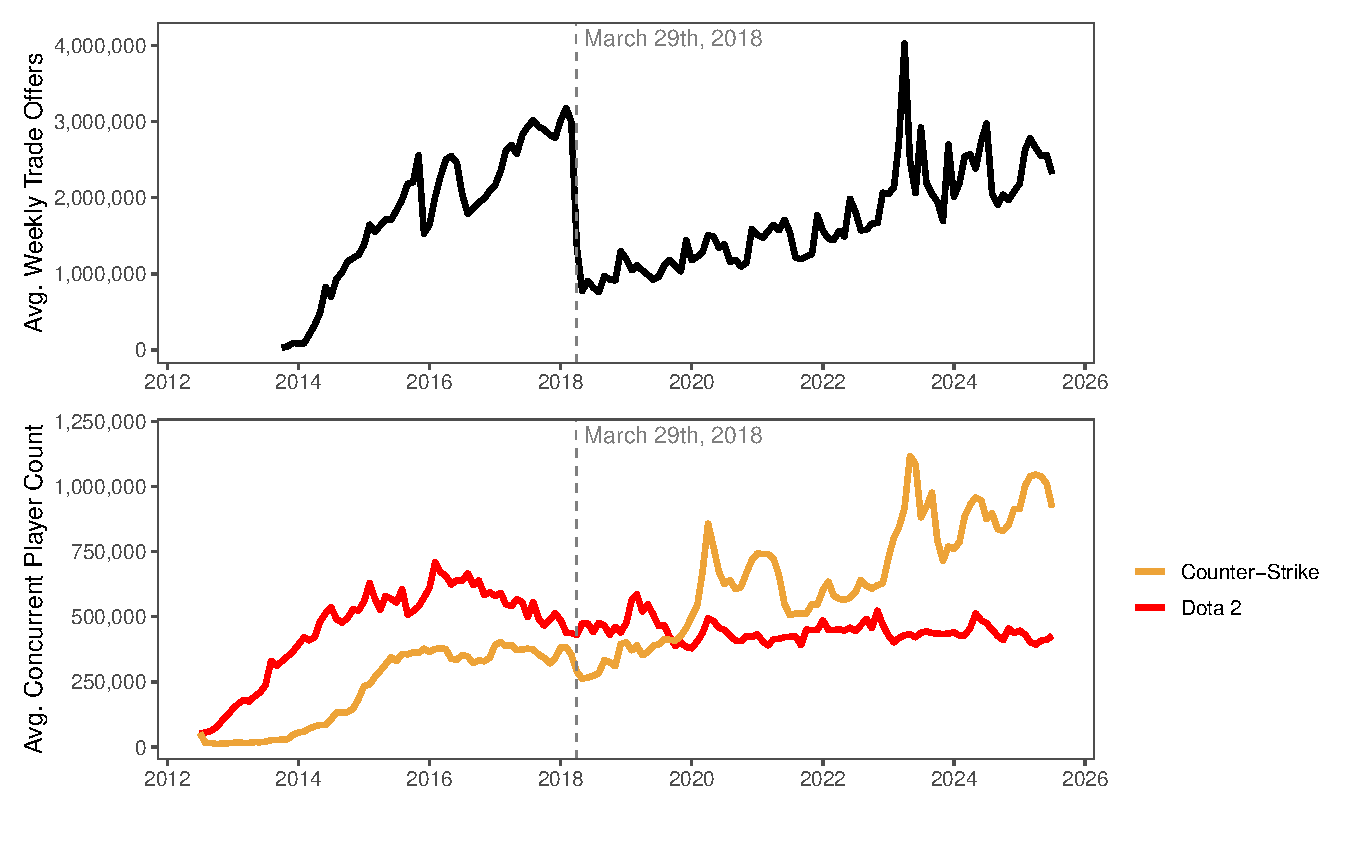
\includegraphics[scale=0.43]{trade_delta_and_plyr_ct.pdf}}

		\raggedright\tiny{\textbf{Note:} Steam trade offer data includes trade offers for all Steam items and is estimated from the difference in trade offer ID between trades. Top chart is sourced from \citeauthor{tradeTF} and bottom figure is sourced from \citeauthor{steamcharts_cs} \nocite{steamcharts_dota}.}
	\end{figure}
\end{frame}
	
%--------------------------------------------------------------------------------------------------
%	DATA & RESULTS
%--------------------------------------------------------------------------------------------------
\section{Data \& Results}
\begin{frame}[shrink=30]{Dataset}
	\begin{table}[h]
	\textbf{Counter-Strike and Dota 2 Items Summary}
	\begin{center}
	\begin{tabular}{lcccc}
	\hline
	                        & Counter-Strike    & Dota 2    & Combined &  \\
	\toprule
	Observations            & 2940          & 2675          & 5615  &  \\
	Unique Items            & 60            & 56            & 116   &  \\
	Oldest Origin Date      & 2013-08-14    & 2014-05-08    & 2013-08-14 &  \\
	Newest Origin Date      & 2016-02-18    & 2016-10-05    & 2016-10-05 &  \\
	Median Sale Price       & \$4.26        & \$1.90        & \$4.13    & \\ 
	                        & (\$7.28)      & (\$3.61)      & (\$7.14) &  \\
	Log Median Sale Price   & 0.517         & -0.064        & 0.484 & \\
	                        & (1.379)       & (1.160)       & (1.253)   & \\
	Volume Sold             & 20524.25      &  1356.84      & 11392.85  & \\ 
	                        & (37685.37)    & (2201.17)     & (28938.78) & \\
	Grade Rarity            & 0.154         & 0.110         & 0.152 & \\ 
	                        & (0.109)       & (0.065)       & (0.107)   & \\
	\bottomrule
	\end{tabular}

	\vspace{2mm}
	\raggedright\footnotesize{\textbf{Note:} Median Price and Grade Rarity are monthly averages weighted by volume sold with weighted standard deviation in parentheses below. Volume Sold is a monthly average with unweighted standard errors. Origin date and grade rarity are provided by \citeauthor{cs2db} and \citeauthor{backpackcs} \nocite{backpackdota} respectively.}
	\end{center}
	\end{table}
\end{frame}

\begin{frame}[shrink=30]{Regressions}
\vspace{5mm}

\textbf{First Stage Hedonic Regression (Quality-Adjustment):}
\begin{equation}
    \log(p_{it}) = \beta_0 + \beta_1 ItemAge_{it} + \beta_2 ItemAge_{it}^2 + \beta_3 GradeRarity_{i} + \beta_4 GradeRarity_{i}^2 + \varepsilon_{it}
\end{equation}

\begin{itemize}
	\item We carry out this first stage regression to control for heterogeneity in item quality.
	\item Individual items can become more or less valuable due to changing taste preferences and/or game updates that modify in-game performance or appearances.
\end{itemize}

\textbf{TWFE Regression:}
\begin{equation}
    \log(\hat{p}_{it}) = \beta_0 + \beta_1 \log(ConcurrentPlayers)_{it} + \delta Treated_i\times Post_t + \underbrace{\alpha_i}_{\text{item FE}} + \underbrace{\gamma_t}_{\text{month FE}} + \varepsilon_{it}
\end{equation}

\textbf{Event Study Regression:}
\begin{equation}
	\log(\hat{p}_{it}) = \beta_0 + \beta_1 \log(ConcurrentPlayers)_{it} + \sum_{k\neq-1}\delta_{k}\cdot\underbrace{\mathds{1}(k=t-e)_{t}}_{\parbox{3.5em}{\scriptsize\centering k months before treatment period e dummies}}\cdot Treated_{i} + \alpha_i + \gamma_t + \varepsilon_{it}
\end{equation}
\end{frame}

\begin{frame}[shrink=35]{Regression Results}
	\begin{table}[ht!]
	  \renewcommand{\arraystretch}{1.25}%
	  \begin{center}
	  \textbf{First Stage Hedonic and TWFE Regression Results}

	  \begin{tabular}[t]{lc}
	    \hline
	     & \(\log(p_{it})\) \\ \toprule
	    \(\beta_0\)         & $1.595^{***}$ \\
	                        & $(0.075)$ \\
	    $ItemAge$           & $0.029^{***}$ \\ 
	                        & $(0.003)$ \\
	    $ItemAge^2$         & $-0.001^{***}$ \\
	                        & $(0.000)$ \\
	    $GradeRarity$       & $-19.43^{***}$ \\ 
	                        & $( 0.894)$ \\
	    $GradeRarity^2$     & $38.37^{***}$ \\
	                        & $(2.623)$ \\ \hline
	    N                   & 5615 \\
	    Adjusted \(R^2\)    & 0.452 \\ 
	    \bottomrule
	  \end{tabular}
	  \quad
	  \begin{tabular}[t]{lcc}
	    \hline
	                                        & \(\log(\hat{p}_{it})\) & \(\log(Volume \: Sold)\) \\ \toprule
	    $\log(ConcurrentPlayers)$           & $-0.050^{***}$         & $-0.422^{***}$ \\ 
	                                        & $(0.012)$              & $(0.120)$ \\
	    $Treated\times Post$                & $-0.043^{***}$         & $-0.326^{***}$ \\
	                                        & $(0.010)$              & $(0.081)$ \\ \hline
	    N                                   & 5579                   & 5615 \\
	    Adjusted \(R^2\)                    & 0.997                  & 0.956 \\
	    Within \(R^2\)                      & 0.130                  & 0.055 \\ \hline
	    Item and Month FEs                  & \checkmark             & \checkmark \\
	    \bottomrule
	  \end{tabular}
	\vspace{2mm}

	{\raggedright \footnotesize{\textbf{Note:} $^{*}\, p<0.5$; $^{**}\, p<0.01$; $^{***}\, p<0.001$. Standard errors are shown in parentheses below their respective estimates. Both regressions with price as a dependent variable are weighted by Volume Sold. Item Age is in terms of months.} \par}
	\vspace{2mm}
	\end{center}
	\end{table}
\end{frame}

\begin{frame}[c]{Event Study Results}
\begin{center}
    \begin{figure}[ht]
        \begin{minipage}[b]{0.45\textwidth}
            \centering
            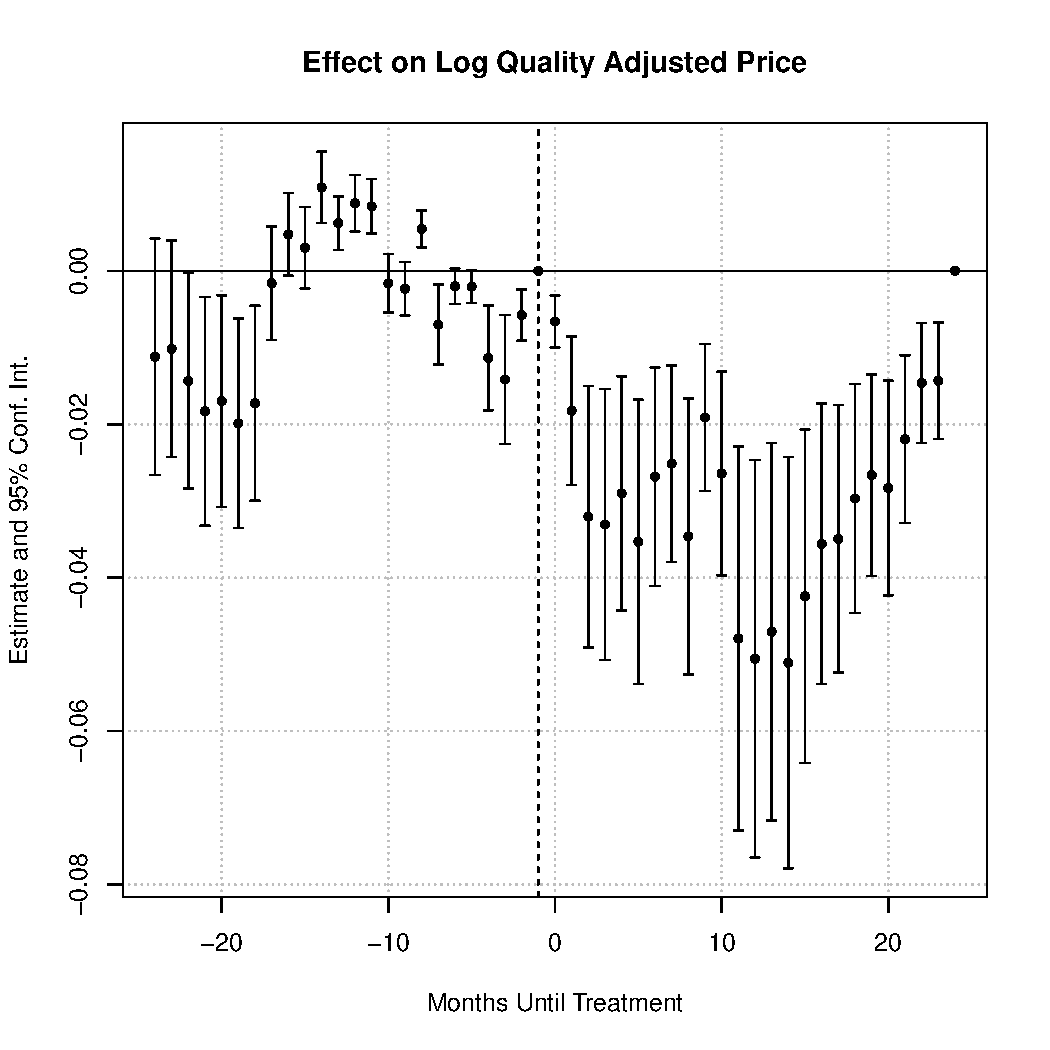
\includegraphics[width=5cm]{did_mos_2yr_phat_iplot.pdf}
        \end{minipage}
		\hfill
        \begin{minipage}[b]{0.45\textwidth}
            \centering
            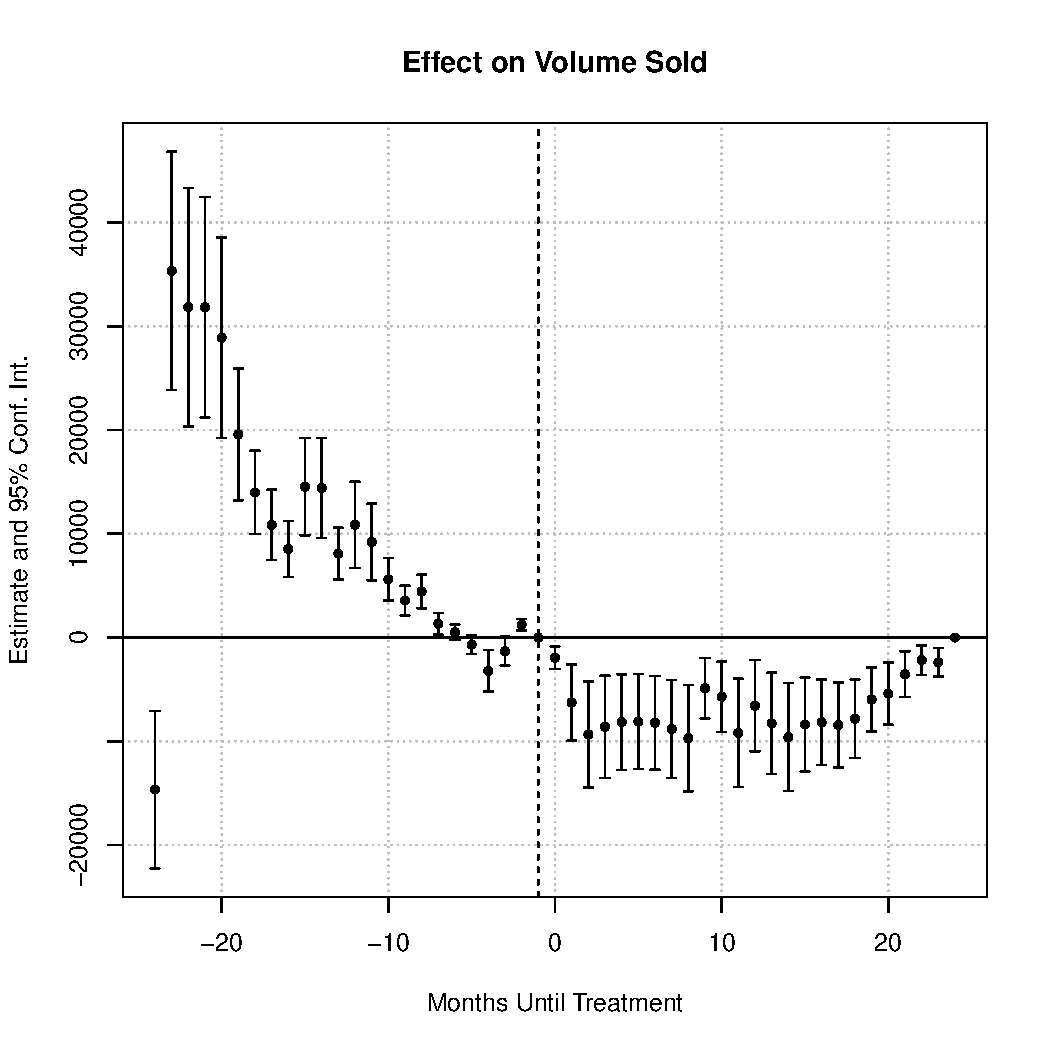
\includegraphics[width=5cm]{did_mos_2yr_vol_iplot.pdf}
        \end{minipage}
    \end{figure}
\tiny{\textbf{Note:} The last period, \(t=24\) is excluded and shown here as 0 due to collinearity.}
\end{center}
\end{frame}


%--------------------------------------------------------------------------------------------------
%	CONCLUSION
%--------------------------------------------------------------------------------------------------
\section{Conclusion}

\begin{frame}{Next Steps}
\begin{itemize}
	\item Additional controls to handle ``seasonality'' in game updates.
	\item Additional troubleshooting on event study design.
	\item Web scrape listed buy orders and offers from the Internet Archive's Wayback Machine.
	\begin{itemize}
		\item Gives us the bid-ask spread which gives us a direct measure of the decline in liquidity.
		\item May provide more insight into the liquidity premium price channel.
		\item Only challenge (besides coding) is endogeneity in data gaps.
	\end{itemize}
	\item Eventually a structural model may help me produce more interpretable estimates. 
\end{itemize}
\end{frame}

\begin{frame}{Conclusion}
	\begin{itemize}
		\item Liquidity plays a key role in determining prices, returns, and choice in physical \underline{and virtual} assets.
		\begin{itemize}
			\item Despite being primarily valued for their aesthetic, Counter-Strike skins faced a 4.2\% illiquidity discount  and 34.4\% decline in trade volume after trade ban implementation.
		\end{itemize}
		\item As online exchanges proliferate, market administrators need to carefully consider market structure.
		\item Virtual markets can serve as valuable sources of high frequency data relating to more traditional ones.
	\end{itemize}
\end{frame}

%--------------------------------------------------------------------------------------------------
%	REFERENCES
%--------------------------------------------------------------------------------------------------

\begin{frame}[allowframebreaks]{References}
    \printbibliography
\end{frame}

\end{document}
